\documentclass{standalone}
\usepackage{tikz}
\usetikzlibrary{patterns, positioning}


\begin{document}
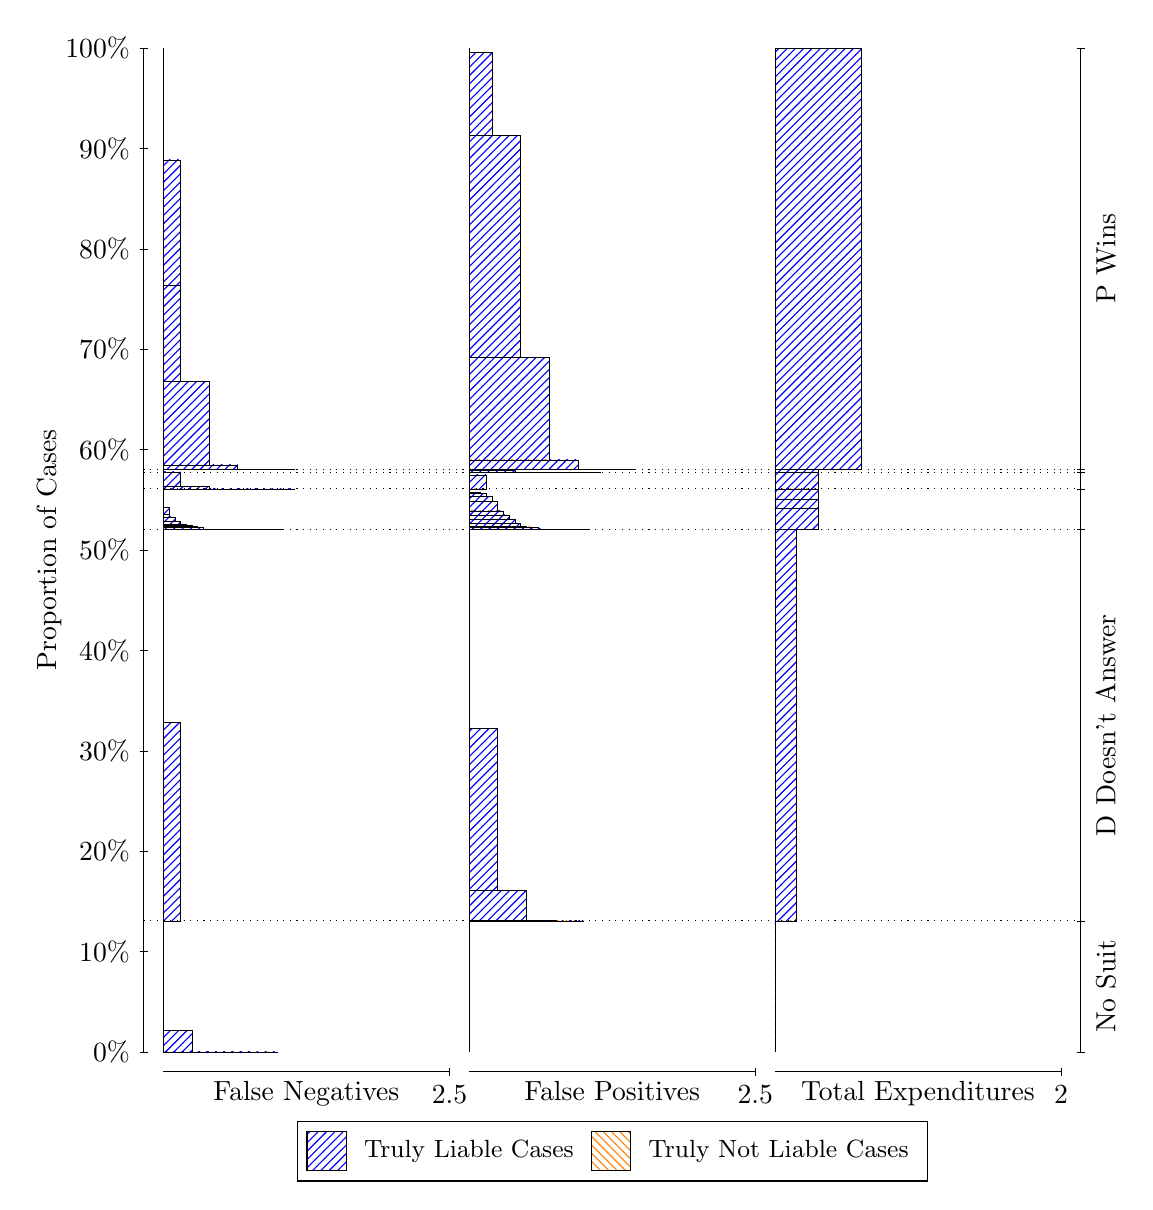
\begin{tikzpicture}
\draw[black, very thin] (1.5,1.75) -- (1.5,14.5);
\node[rotate=90, text=black, anchor=center] at (0.3, 8.125) {Proportion of Cases};
\draw[black, very thin] (1.45,1.75) -- (1.55,1.75);
\node[text=black, anchor=east] at (1.45, 1.75) {0\%};
\draw[black, very thin] (1.45,3.025) -- (1.55,3.025);
\node[text=black, anchor=east] at (1.45, 3.025) {10\%};
\draw[black, very thin] (1.45,4.3) -- (1.55,4.3);
\node[text=black, anchor=east] at (1.45, 4.3) {20\%};
\draw[black, very thin] (1.45,5.575) -- (1.55,5.575);
\node[text=black, anchor=east] at (1.45, 5.575) {30\%};
\draw[black, very thin] (1.45,6.85) -- (1.55,6.85);
\node[text=black, anchor=east] at (1.45, 6.85) {40\%};
\draw[black, very thin] (1.45,8.125) -- (1.55,8.125);
\node[text=black, anchor=east] at (1.45, 8.125) {50\%};
\draw[black, very thin] (1.45,9.4) -- (1.55,9.4);
\node[text=black, anchor=east] at (1.45, 9.4) {60\%};
\draw[black, very thin] (1.45,10.675) -- (1.55,10.675);
\node[text=black, anchor=east] at (1.45, 10.675) {70\%};
\draw[black, very thin] (1.45,11.95) -- (1.55,11.95);
\node[text=black, anchor=east] at (1.45, 11.95) {80\%};
\draw[black, very thin] (1.45,13.225) -- (1.55,13.225);
\node[text=black, anchor=east] at (1.45, 13.225) {90\%};
\draw[black, very thin] (1.45,14.5) -- (1.55,14.5);
\node[text=black, anchor=east] at (1.45, 14.5) {100\%};

\draw[black, very thin] (13.4,1.75) -- (13.4,14.5);
\draw[black, very thin] (13.35,1.75) -- (13.45,1.75);
\node[anchor=west] at (13.35, 1.75) {};
\draw[black, very thin] (13.35,3.4152) -- (13.45,3.4152);
\node[anchor=west] at (13.35, 3.4152) {};
\draw[black, very thin] (13.35,8.3867) -- (13.45,8.3867);
\node[anchor=west] at (13.35, 8.3867) {};
\draw[black, very thin] (13.35,8.9019) -- (13.45,8.9019);
\node[anchor=west] at (13.35, 8.9019) {};
\draw[black, very thin] (13.35,9.1096) -- (13.45,9.1096);
\node[anchor=west] at (13.35, 9.1096) {};
\draw[black, very thin] (13.35,9.1517) -- (13.45,9.1517);
\node[anchor=west] at (13.35, 9.1517) {};
\draw[black, very thin] (13.35,14.5) -- (13.45,14.5);
\node[anchor=west] at (13.35, 14.5) {};

\draw[black, very thin, pattern color=blue, pattern=north east lines] (1.75,1.75) rectangle (3.2033,1.75);
\draw[black, very thin, pattern color=blue, pattern=north east lines] (1.75,1.75) rectangle (2.84,1.75);
\draw[black, very thin, pattern color=blue, pattern=north east lines] (1.75,1.75) rectangle (2.4767,1.7523);
\draw[black, very thin, pattern color=blue, pattern=north east lines] (1.75,1.7523) rectangle (2.1133,2.0227);
\draw[black, very thin, pattern color=orange, pattern=north west lines] (1.75,2.0227) rectangle (1.75,2.0227);
\draw[black, very thin, pattern color=blue, pattern=north east lines] (1.75,2.0227) rectangle (1.75,3.4152);
\draw[black, very thin, pattern color=blue, pattern=north east lines] (1.75,3.4152) rectangle (1.968,5.938);
\draw[black, very thin, pattern color=orange, pattern=north west lines] (1.75,5.938) rectangle (1.75,5.938);
\draw[black, very thin, pattern color=blue, pattern=north east lines] (1.75,5.938) rectangle (1.75,8.3867);
\draw[black, very thin, pattern color=blue, pattern=north east lines] (1.75,8.3867) rectangle (3.276,8.3867);
\draw[black, very thin, pattern color=blue, pattern=north east lines] (1.75,8.3867) rectangle (3.1307,8.3867);
\draw[black, very thin, pattern color=blue, pattern=north east lines] (1.75,8.3867) rectangle (2.9853,8.3867);
\draw[black, very thin, pattern color=blue, pattern=north east lines] (1.75,8.3867) rectangle (2.9127,8.3867);
\draw[black, very thin, pattern color=blue, pattern=north east lines] (1.75,8.3867) rectangle (2.84,8.3867);
\draw[black, very thin, pattern color=blue, pattern=north east lines] (1.75,8.3867) rectangle (2.7673,8.3867);
\draw[black, very thin, pattern color=blue, pattern=north east lines] (1.75,8.3867) rectangle (2.6947,8.3867);
\draw[black, very thin, pattern color=blue, pattern=north east lines] (1.75,8.3867) rectangle (2.622,8.3868);
\draw[black, very thin, pattern color=blue, pattern=north east lines] (1.75,8.3868) rectangle (2.5493,8.3868);
\draw[black, very thin, pattern color=blue, pattern=north east lines] (1.75,8.3868) rectangle (2.4767,8.3868);
\draw[black, very thin, pattern color=blue, pattern=north east lines] (1.75,8.3868) rectangle (2.404,8.3869);
\draw[black, very thin, pattern color=blue, pattern=north east lines] (1.75,8.3869) rectangle (2.404,8.387);
\draw[black, very thin, pattern color=blue, pattern=north east lines] (1.75,8.387) rectangle (2.3313,8.3885);
\draw[black, very thin, pattern color=blue, pattern=north east lines] (1.75,8.3885) rectangle (2.2587,8.4084);
\draw[black, very thin, pattern color=blue, pattern=north east lines] (1.75,8.4084) rectangle (2.186,8.4099);
\draw[black, very thin, pattern color=blue, pattern=north east lines] (1.75,8.4099) rectangle (2.186,8.4247);
\draw[black, very thin, pattern color=blue, pattern=north east lines] (1.75,8.4247) rectangle (2.1133,8.4369);
\draw[black, very thin, pattern color=blue, pattern=north east lines] (1.75,8.4369) rectangle (2.0407,8.4424);
\draw[black, very thin, pattern color=blue, pattern=north east lines] (1.75,8.4424) rectangle (2.0407,8.4465);
\draw[black, very thin, pattern color=blue, pattern=north east lines] (1.75,8.4465) rectangle (1.968,8.4853);
\draw[black, very thin, pattern color=blue, pattern=north east lines] (1.75,8.4853) rectangle (1.8953,8.5445);
\draw[black, very thin, pattern color=blue, pattern=north east lines] (1.75,8.5445) rectangle (1.8953,8.5462);
\draw[black, very thin, pattern color=blue, pattern=north east lines] (1.75,8.5462) rectangle (1.8227,8.5737);
\draw[black, very thin, pattern color=blue, pattern=north east lines] (1.75,8.5737) rectangle (1.8227,8.6667);
\draw[black, very thin, pattern color=blue, pattern=north east lines] (1.75,8.6667) rectangle (1.75,8.6671);
\draw[black, very thin, pattern color=orange, pattern=north west lines] (1.75,8.6671) rectangle (1.75,8.6671);
\draw[black, very thin, pattern color=blue, pattern=north east lines] (1.75,8.6671) rectangle (1.75,8.9019);
\draw[black, very thin, pattern color=blue, pattern=north east lines] (1.75,8.9019) rectangle (3.4213,8.9019);
\draw[black, very thin, pattern color=blue, pattern=north east lines] (1.75,8.9019) rectangle (3.058,8.9019);
\draw[black, very thin, pattern color=blue, pattern=north east lines] (1.75,8.9019) rectangle (2.6947,8.9021);
\draw[black, very thin, pattern color=blue, pattern=north east lines] (1.75,8.9021) rectangle (2.3313,8.9338);
\draw[black, very thin, pattern color=blue, pattern=north east lines] (1.75,8.9338) rectangle (1.968,9.1096);
\draw[black, very thin, pattern color=orange, pattern=north west lines] (1.75,9.1096) rectangle (1.75,9.1096);
\draw[black, very thin, pattern color=blue, pattern=north east lines] (1.75,9.1096) rectangle (1.968,9.1175);
\draw[black, very thin, pattern color=orange, pattern=north west lines] (1.75,9.1175) rectangle (1.75,9.1175);
\draw[black, very thin, pattern color=blue, pattern=north east lines] (1.75,9.1175) rectangle (1.75,9.1517);
\draw[black, very thin, pattern color=blue, pattern=north east lines] (1.75,9.1517) rectangle (3.4213,9.1517);
\draw[black, very thin, pattern color=blue, pattern=north east lines] (1.75,9.1517) rectangle (3.058,9.1519);
\draw[black, very thin, pattern color=blue, pattern=north east lines] (1.75,9.1519) rectangle (2.6947,9.2073);
\draw[black, very thin, pattern color=blue, pattern=north east lines] (1.75,9.2073) rectangle (2.3313,10.262);
\draw[black, very thin, pattern color=blue, pattern=north east lines] (1.75,10.262) rectangle (1.968,11.489);
\draw[black, very thin, pattern color=blue, pattern=north east lines] (1.75,11.489) rectangle (1.968,13.079);
\draw[black, very thin, pattern color=orange, pattern=north west lines] (1.75,13.079) rectangle (1.75,13.079);
\draw[black, very thin, pattern color=blue, pattern=north east lines] (1.75,13.079) rectangle (1.75,14.5);
\draw[black, very thin, pattern color=orange, pattern=north west lines] (5.6333,1.75) rectangle (5.6333,1.75);
\draw[black, very thin, pattern color=blue, pattern=north east lines] (5.6333,1.75) rectangle (5.6333,3.4152);
\draw[black, very thin, pattern color=orange, pattern=north west lines] (5.6333,3.4152) rectangle (7.0867,3.4152);
\draw[black, very thin, pattern color=blue, pattern=north east lines] (5.6333,3.4152) rectangle (7.0867,3.4152);
\draw[black, very thin, pattern color=blue, pattern=north east lines] (5.6333,3.4152) rectangle (6.7233,3.4181);
\draw[black, very thin, pattern color=blue, pattern=north east lines] (5.6333,3.4181) rectangle (6.36,3.803);
\draw[black, very thin, pattern color=blue, pattern=north east lines] (5.6333,3.803) rectangle (5.9967,5.8639);
\draw[black, very thin, pattern color=blue, pattern=north east lines] (5.6333,5.8639) rectangle (5.6333,8.3867);
\draw[black, very thin, pattern color=orange, pattern=north west lines] (5.6333,8.3867) rectangle (7.1593,8.3867);
\draw[black, very thin, pattern color=blue, pattern=north east lines] (5.6333,8.3867) rectangle (7.1593,8.3867);
\draw[black, very thin, pattern color=orange, pattern=north west lines] (5.6333,8.3867) rectangle (7.014,8.3867);
\draw[black, very thin, pattern color=blue, pattern=north east lines] (5.6333,8.3867) rectangle (7.014,8.3867);
\draw[black, very thin, pattern color=orange, pattern=north west lines] (5.6333,8.3867) rectangle (6.8687,8.3867);
\draw[black, very thin, pattern color=blue, pattern=north east lines] (5.6333,8.3867) rectangle (6.8687,8.3868);
\draw[black, very thin, pattern color=blue, pattern=north east lines] (5.6333,8.3868) rectangle (6.796,8.3868);
\draw[black, very thin, pattern color=orange, pattern=north west lines] (5.6333,8.3868) rectangle (6.7233,8.3868);
\draw[black, very thin, pattern color=blue, pattern=north east lines] (5.6333,8.3868) rectangle (6.7233,8.3868);
\draw[black, very thin, pattern color=blue, pattern=north east lines] (5.6333,8.3868) rectangle (6.6507,8.3869);
\draw[black, very thin, pattern color=orange, pattern=north west lines] (5.6333,8.3869) rectangle (6.578,8.3869);
\draw[black, very thin, pattern color=blue, pattern=north east lines] (5.6333,8.3869) rectangle (6.578,8.3929);
\draw[black, very thin, pattern color=blue, pattern=north east lines] (5.6333,8.3929) rectangle (6.5053,8.4098);
\draw[black, very thin, pattern color=orange, pattern=north west lines] (5.6333,8.4098) rectangle (6.4327,8.4098);
\draw[black, very thin, pattern color=blue, pattern=north east lines] (5.6333,8.4098) rectangle (6.4327,8.4192);
\draw[black, very thin, pattern color=orange, pattern=north west lines] (5.6333,8.4192) rectangle (6.4327,8.4192);
\draw[black, very thin, pattern color=blue, pattern=north east lines] (5.6333,8.4192) rectangle (6.4327,8.4193);
\draw[black, very thin, pattern color=blue, pattern=north east lines] (5.6333,8.4193) rectangle (6.36,8.4265);
\draw[black, very thin, pattern color=blue, pattern=north east lines] (5.6333,8.4265) rectangle (6.2873,8.4274);
\draw[black, very thin, pattern color=orange, pattern=north west lines] (5.6333,8.4274) rectangle (6.2873,8.4274);
\draw[black, very thin, pattern color=blue, pattern=north east lines] (5.6333,8.4274) rectangle (6.2873,8.4664);
\draw[black, very thin, pattern color=blue, pattern=north east lines] (5.6333,8.4664) rectangle (6.2147,8.5129);
\draw[black, very thin, pattern color=orange, pattern=north west lines] (5.6333,8.5129) rectangle (6.142,8.5129);
\draw[black, very thin, pattern color=blue, pattern=north east lines] (5.6333,8.5129) rectangle (6.142,8.5699);
\draw[black, very thin, pattern color=blue, pattern=north east lines] (5.6333,8.5699) rectangle (6.0693,8.6216);
\draw[black, very thin, pattern color=blue, pattern=north east lines] (5.6333,8.6216) rectangle (6.0693,8.622);
\draw[black, very thin, pattern color=orange, pattern=north west lines] (5.6333,8.622) rectangle (5.9967,8.622);
\draw[black, very thin, pattern color=blue, pattern=north east lines] (5.6333,8.622) rectangle (5.9967,8.7425);
\draw[black, very thin, pattern color=blue, pattern=north east lines] (5.6333,8.7425) rectangle (5.924,8.7442);
\draw[black, very thin, pattern color=blue, pattern=north east lines] (5.6333,8.7442) rectangle (5.924,8.8033);
\draw[black, very thin, pattern color=blue, pattern=north east lines] (5.6333,8.8033) rectangle (5.8513,8.8422);
\draw[black, very thin, pattern color=blue, pattern=north east lines] (5.6333,8.8422) rectangle (5.7787,8.8518);
\draw[black, very thin, pattern color=blue, pattern=north east lines] (5.6333,8.8518) rectangle (5.706,8.8639);
\draw[black, very thin, pattern color=blue, pattern=north east lines] (5.6333,8.8639) rectangle (5.706,8.8639);
\draw[black, very thin, pattern color=blue, pattern=north east lines] (5.6333,8.8639) rectangle (5.6333,8.9019);
\draw[black, very thin, pattern color=orange, pattern=north west lines] (5.6333,8.9019) rectangle (5.8513,8.9019);
\draw[black, very thin, pattern color=blue, pattern=north east lines] (5.6333,8.9019) rectangle (5.8513,9.0777);
\draw[black, very thin, pattern color=blue, pattern=north east lines] (5.6333,9.0777) rectangle (5.6333,9.1096);
\draw[black, very thin, pattern color=orange, pattern=north west lines] (5.6333,9.1096) rectangle (7.3047,9.1096);
\draw[black, very thin, pattern color=blue, pattern=north east lines] (5.6333,9.1096) rectangle (7.3047,9.1096);
\draw[black, very thin, pattern color=blue, pattern=north east lines] (5.6333,9.1096) rectangle (6.9413,9.1096);
\draw[black, very thin, pattern color=blue, pattern=north east lines] (5.6333,9.1096) rectangle (6.578,9.1155);
\draw[black, very thin, pattern color=blue, pattern=north east lines] (5.6333,9.1155) rectangle (6.2147,9.1438);
\draw[black, very thin, pattern color=blue, pattern=north east lines] (5.6333,9.1438) rectangle (5.8513,9.1517);
\draw[black, very thin, pattern color=orange, pattern=north west lines] (5.6333,9.1517) rectangle (7.7407,9.1517);
\draw[black, very thin, pattern color=blue, pattern=north east lines] (5.6333,9.1517) rectangle (7.7407,9.1517);
\draw[black, very thin, pattern color=orange, pattern=north west lines] (5.6333,9.1517) rectangle (7.3773,9.1517);
\draw[black, very thin, pattern color=blue, pattern=north east lines] (5.6333,9.1517) rectangle (7.3773,9.1531);
\draw[black, very thin, pattern color=orange, pattern=north west lines] (5.6333,9.1531) rectangle (7.014,9.1531);
\draw[black, very thin, pattern color=blue, pattern=north east lines] (5.6333,9.1531) rectangle (7.014,9.2699);
\draw[black, very thin, pattern color=orange, pattern=north west lines] (5.6333,9.2699) rectangle (6.6507,9.2699);
\draw[black, very thin, pattern color=blue, pattern=north east lines] (5.6333,9.2699) rectangle (6.6507,10.573);
\draw[black, very thin, pattern color=orange, pattern=north west lines] (5.6333,10.573) rectangle (6.2873,10.573);
\draw[black, very thin, pattern color=blue, pattern=north east lines] (5.6333,10.573) rectangle (6.2873,13.39);
\draw[black, very thin, pattern color=blue, pattern=north east lines] (5.6333,13.39) rectangle (5.924,14.444);
\draw[black, very thin, pattern color=blue, pattern=north east lines] (5.6333,14.444) rectangle (5.6333,14.5);
\draw[black, very thin, pattern color=orange, pattern=north west lines] (9.5167,1.75) rectangle (9.5167,1.75);
\draw[black, very thin, pattern color=blue, pattern=north east lines] (9.5167,1.75) rectangle (9.5167,3.4152);
\draw[black, very thin, pattern color=orange, pattern=north west lines] (9.5167,3.4152) rectangle (9.7892,3.4152);
\draw[black, very thin, pattern color=blue, pattern=north east lines] (9.5167,3.4152) rectangle (9.7892,8.3867);
\draw[black, very thin, pattern color=orange, pattern=north west lines] (9.5167,8.3867) rectangle (10.062,8.3867);
\draw[black, very thin, pattern color=blue, pattern=north east lines] (9.5167,8.3867) rectangle (10.062,8.6555);
\draw[black, very thin, pattern color=orange, pattern=north west lines] (9.5167,8.6555) rectangle (10.062,8.6555);
\draw[black, very thin, pattern color=blue, pattern=north east lines] (9.5167,8.6555) rectangle (10.062,8.7634);
\draw[black, very thin, pattern color=orange, pattern=north west lines] (9.5167,8.7634) rectangle (10.062,8.7634);
\draw[black, very thin, pattern color=blue, pattern=north east lines] (9.5167,8.7634) rectangle (10.062,8.9019);
\draw[black, very thin, pattern color=orange, pattern=north west lines] (9.5167,8.9019) rectangle (10.062,8.9019);
\draw[black, very thin, pattern color=blue, pattern=north east lines] (9.5167,8.9019) rectangle (10.062,9.1096);
\draw[black, very thin, pattern color=orange, pattern=north west lines] (9.5167,9.1096) rectangle (10.062,9.1096);
\draw[black, very thin, pattern color=blue, pattern=north east lines] (9.5167,9.1096) rectangle (10.062,9.1517);
\draw[black, very thin, pattern color=orange, pattern=north west lines] (9.5167,9.1517) rectangle (10.607,9.1517);
\draw[black, very thin, pattern color=blue, pattern=north east lines] (9.5167,9.1517) rectangle (10.607,14.5);
\draw[black, dotted] (1.5,3.4152) -- (13.4,3.4152);
\draw[black, dotted] (1.5,8.3867) -- (13.4,8.3867);
\draw[black, dotted] (1.5,8.9019) -- (13.4,8.9019);
\draw[black, dotted] (1.5,9.1096) -- (13.4,9.1096);
\draw[black, dotted] (1.5,9.1517) -- (13.4,9.1517);
\draw[black, very thin] (1.75,1.5) -- (5.3833,1.5);
\node[text=black, anchor=north] at (3.5667, 1.5) {False Negatives};
\draw[black, very thin] (5.3833,1.45) -- (5.3833,1.55);
\node[text=black, anchor=north] at (5.3833, 1.45) {2.5};

\draw[black, very thin] (5.6333,1.5) -- (9.2667,1.5);
\node[text=black, anchor=north] at (7.45, 1.5) {False Positives};
\draw[black, very thin] (9.2667,1.45) -- (9.2667,1.55);
\node[text=black, anchor=north] at (9.2667, 1.45) {2.5};

\draw[black, very thin] (9.5167,1.5) -- (13.15,1.5);
\node[text=black, anchor=north] at (11.333, 1.5) {Total Expenditures};
\draw[black, very thin] (13.15,1.45) -- (13.15,1.55);
\node[text=black, anchor=north] at (13.15, 1.45) {2};

\node[text=black, centered, rotate=90] at (13.72, 2.5826) {No Suit};
\node[text=black, centered, rotate=90] at (13.72, 5.901) {D Doesn't Answer};



\node[text=black, centered, rotate=90] at (13.72, 11.826) {P Wins};

\draw (7.449999999999999,1.5) node[draw=none] (baseCoordinate) {};
\begin{scope}[align=center]
        \matrix[scale=0.5, draw=black, below=0.5cm of baseCoordinate, nodes={draw}, column sep=0.1cm]{
            \node[rectangle, draw, minimum width=0.5cm, minimum height=0.5cm, pattern color=blue, pattern=north east lines] {}; &
            \node[draw=none, font=\small, text=black] (B) {Truly Liable Cases}; &
            \node[rectangle, draw, minimum width=0.5cm, minimum height=0.5cm, pattern color=orange, pattern=north west lines] {}; &
            \node[draw=none, font=\small, text=black] (B) {Truly Not Liable Cases}; \\
            };
\end{scope}

\end{tikzpicture}
\end{document}